\section{Durchführung}
\label{sec:Durchfuehrung}
Die verwendete Wärmepumpe ist in Abbildung \ref{fig:pumpe} dargestellt.
\begin{figure}
	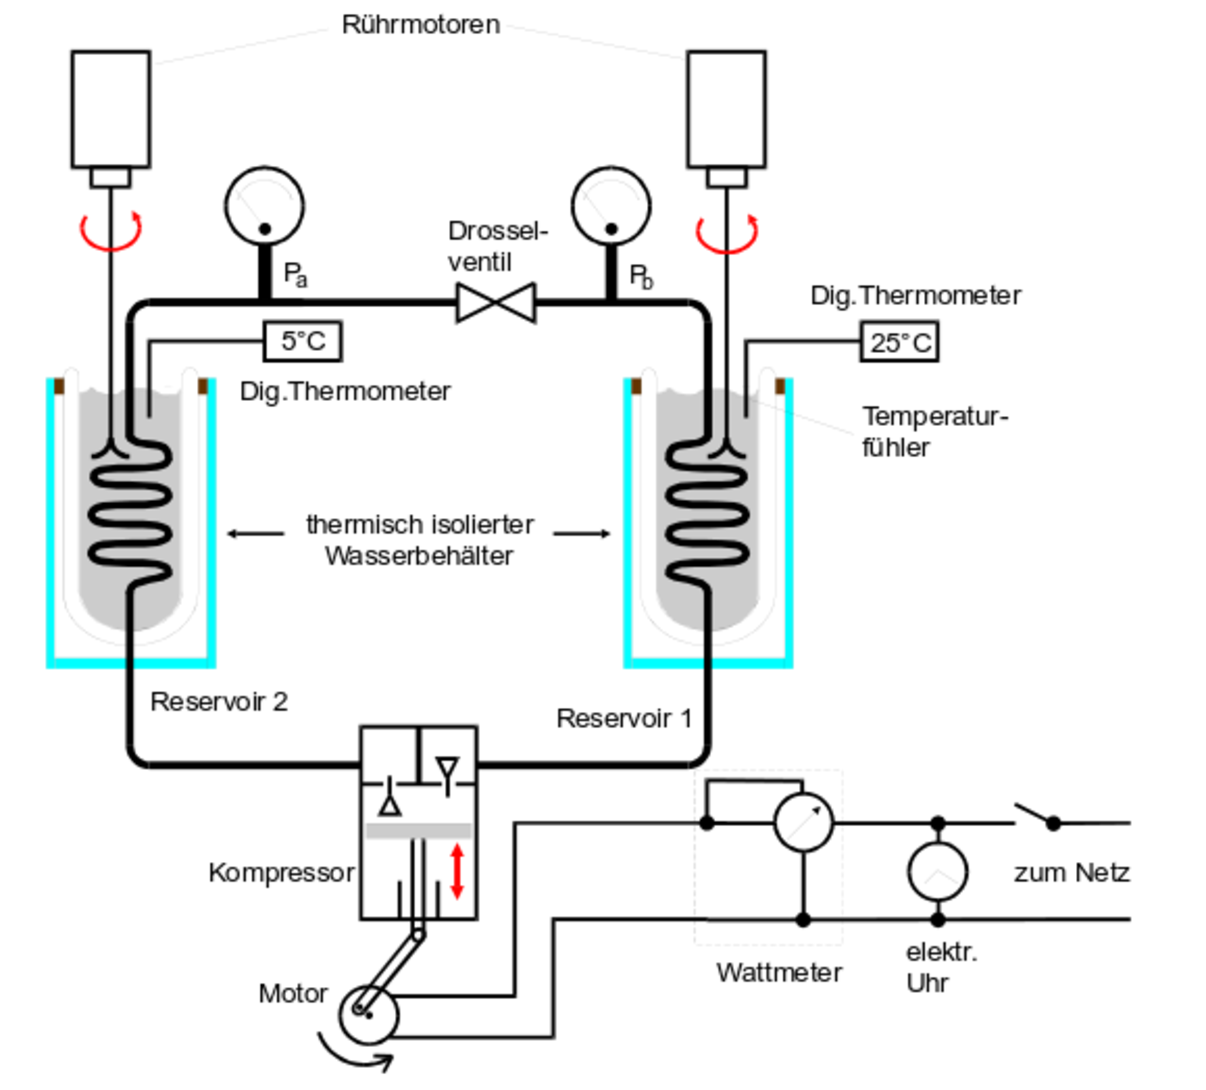
\includegraphics[width=\textwidth]{Bilder/Abbildung.pdf}
	\caption{Schematischer Aufbau der Wärmepumpe \cite{V206}}
	\label{fig:pumpe}
\end{figure}
Durch das geschlossene System fließt eine Medium mit hoher Kondensationswärme, etwa eine Flüssigkeit der FCKW-Gruppe.
Das Medium verdampft in der Kupferschlange im kühlen Reservoir bei geringem Druck $p_a$ und wird im Kompressor adiabatisch komprimiert. 
Das Gas wird unter höherem Druck $p_b$ zum warmen Reservoir geführt und kondensiert in dessen Kupferschlange unter Abgabe der aufgenommenen Energie $Q_2+A$.
Das Drosselventil sorgt für einen Druckunterschied im Kreislauf, sodass die Flüssigkeit erneut unter dem geringerem Druck $p_a$ in der Kupferschlange des kühlen Reservoirs verdampft. 

Der Kompressor bezieht Energie aus dem Netz, die Leistung des Kompressors wird von einem Wattmeter angezeigt. 
Die Reservoire und die Verbindungsleitungen sind thermisch isoliert, sodass das Wärmepumpensystem abgesehen durch die Kupferschlangen keine Wärme nach außen abgibt.
Während der Messung wird der Inhalt der Reservoire mittels Rührer durchmischt. Die Temperatur des Reservoirs und der Druck in den Kupferschlangen ist per Anzeige ablesbar.

Es wird in den Reservoiren jeweils 3 Liter Leitungswasser mit gleicher Temperatur gefüllt und die Parameter $p_k$, $p_w$, $T_k$, $T_w$ sowie die Leistungsaufnahme des Kompressors $P_\text{el}$ pro Minute aufgenommen.